% ==========================================
% Thesis Report - Prerequisits ( hullb2/brods1 )
% ==========================================

\chapter{Prerequisits}

\section{Eurographics 2009}
After reading a lot of papers about Parallel Rendering, Equalizer, \gls{osg}, \gls{ogre}, etc. we got in contact with some people in the Equalizer community. The fact that the developer of Equalizer, Stefan Eilemann, was already known to the \gls{cpvr} research group guided some ways. We knew there was already some work in progress concerning the combination of a scene graph with Equalizer, meaning \gls{osg} as well as \gls{ogre}. We thought, it was not a bad idea to ask him about his opinion, since the required features for our work were fulfilled in both of the frameworks. The response we got was better than we could have hoped: He named us a group of students from the University of Siegen, Germany, who were working on an integration of \gls{osg} in Equalizer, and he declared himself ready to comply with introducing us to them. Better yet, he suggested we should come to the upcoming conference \emph{Eurographics 2009} taking place in Munich only three weeks later. He would be there having a Birds-Of-a-Feather meeting. The people from the University of Siegen would be there, too. 
After some discussions, we decided to go there for at least two days. The meeting was on Tuesday with the option of another one on Wednesday if there should be more to discuss.
Besides the meeting itself, there were a lot of other interesting events, mostly paper sessions. The \gls{bof} meeting was a success, there were a lot more people than expected and a lot of them showed their interests in an integration of \gls{osg} in Equalizer. There were quite a lot of people from Siegen and we were introduced to the developers and exchanged contact information. Another group, some PHD students from the University of Zurich were present too and it turned out, that they were interested in the project too. 


% Brods1
\section{CAVE Clone}
Because of limited \gls{cave} resources and some student overpopulation we needed to setup an environment similar to the \gls{cave} in order to test our framework. To setup a clone of the \gls{cave}, we needed at least one workstation with enough graphics cards so that we could connect four displays to simulate each \gls{cave} wall. This was enough for a first setup, but we had to keep in mind, that we would have to connect eight projectors afterwards. Therefore, it seemed to be a good start, if we tried it with four graphics cards. Since we were going to render quite a lot of graphics stuff, it could not harm to have a few gigabites of memory and a Quadcore \gls{cpu}. Our framework should run cross-platform at least under Windows XP and a Linux distribution, therefore we needed a harddisk with enough free space for multiple operating systems. By then, we had a table with the following components on it:
\begin{itemize}
	\item Mainboard 
	\item \gls{cpu}
	\item 16 GB Ram
	\item 500 GB Harddisk
	\item 4 x NVidia Quadro FX 1700
	\item 4 Displays
\end{itemize}

At the beginning, we wanted to reuse an old computer case which we got from the BFH-TI IT Support. But soon, we had to realise, that the power supply unit was too weak for the brand-new mainboard. We ordered a new one which consequently did not fit into the old computer case. Hence, we had to buy a new computer case as well. 
The result of our \gls{cave} clone can be seen in Figure \ref{fig:cave_clone}.

\begin{figure}[H]
	\centering
	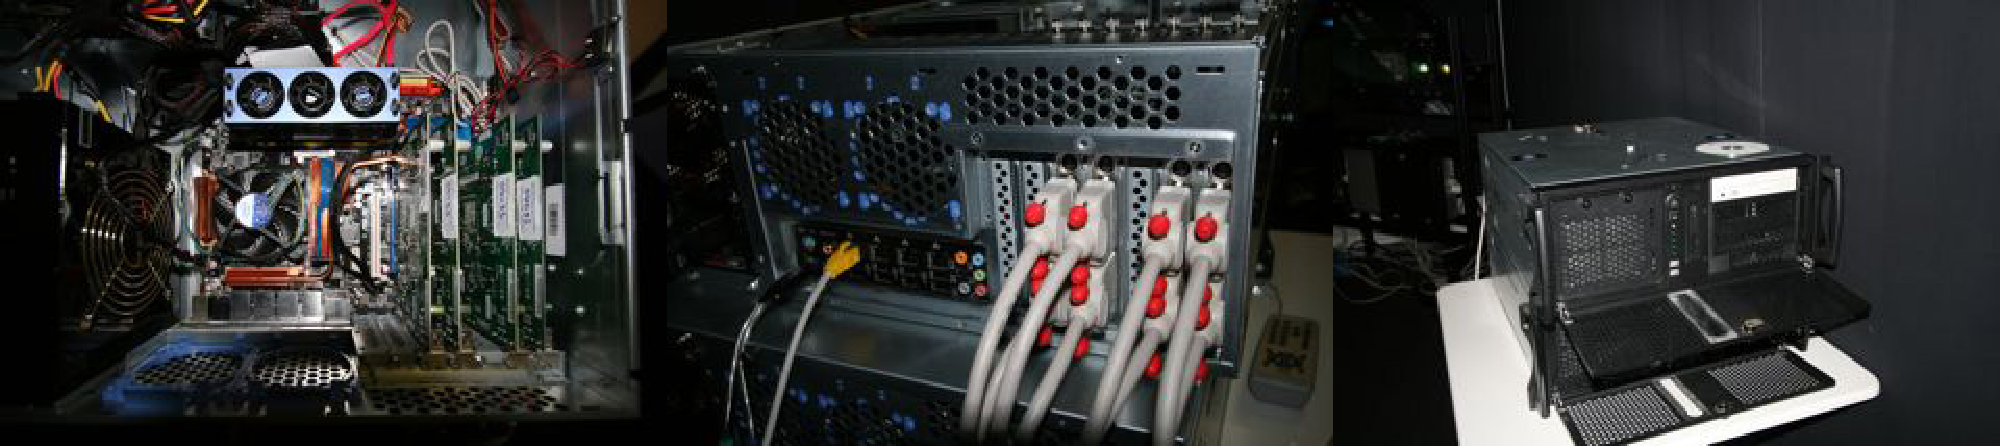
\includegraphics[width=1\textwidth]{../figures/fotos/cave_clone}
	\caption{Cave Clone}
	\label{fig:cave_clone}
\end{figure}

\begin{figure}[H]
	\centering
	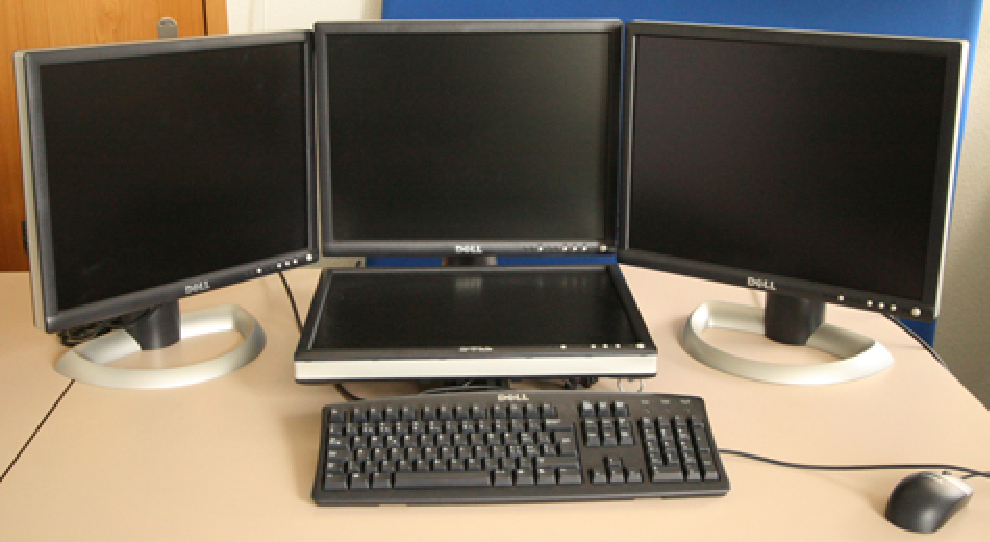
\includegraphics[width=0.4\textwidth]{../figures/fotos/display_setup}
	\caption{Display setup for the CAVE clone}
	\label{fig:displaySetup}
\end{figure}

The 4 displays were arranged in a small cube to simulate the \gls{cave} environment as shown in figure \ref{fig:displaySetup}. 

After screwing it together, we decided to install a dualboot with Windows Vista and Ubuntu 8.10 on it. 

\subsection{Linux Setup}
Detecting the four displays did work right away. We were surprised by that, only a few years earlier, it was quite a challenge to setup more than one display in a linux. The biggest problem was to arrange the four displays in the right order with the right resolution. It pointed out that the NVIDIA driver somhow mixed up the xorg settings of the resolution with some intern stuff. It seemed to be a bug.

Setting up \gls{osg} on Linux was a challenge at first. There are quite a lot of dependencies you have to look after. And soon we realized, that the website of \gls{osg} contains a lot of information, but not really organised, so finding the right dependencies on the list was not that easy. Furthermore, the \gls{osg} version in the aptitude tree of Ubuntu was really old and therefore not usable for our purpose. Finally, we got it running.

To install Equalizer was not that difficult. After about an hour, we could test the first Equalizer application with the default configuration.

Since Equalizer comes with a few sample configurations - amongst other some for multiple pipes - we tried to setup a configuration with four pipes\footnote{A pipe is an Equalizer abstraction for a \gls{gpu}. Consult the \emph{Technical Report} for further information}, for each display one pipe. We could even say which pipe to use for which display. So, it seemed we had a running linux setup.

\subsection{Windows Vista Setup}
Detecting multiple displays in a Windows system is done fast. Therefore, we could straight go on to install \gls{osg} and Equalizer. After we got rid of the Windows Vista security settings which ask you for everything before doing it and consequently skips installing something in the Windows system directories, we could install OSG and Equalizer without any further problems. 
The test application of Equalizer ran without any problems. But as soon as we tried our new configuration file which specified four different pipes, the operating system crashed. We figured out that we could run an application on all four displays, as long as we did not specify any pipes. But it seemed as if all the rendering was done on the \gls{cpu} instead of the \glspl{gpu} and therefore the application ran on a terrible framerate.
After a few hours, we tried to use only one pipe for all four displays. It appeared that this worked and the rendering was no longer done on the \gls{cpu} but only on one \gls{gpu} (what was expected, since we specified this in the configuration file). Therefore, we had a partial success. So we tried to simply use another graphics card. This did not work any more, the result was quite strange, the application started, but it hat about 10 times longer than with the first \gls{gpu} and the windows on the displays were all empty.
Using the third \gls{gpu} did bring on another problem again - here the displays were all black. We could not and still can not explain this surprising behaviour. We figured out, that Windows Vista is not really designed to use multiple graphics cards. And Equalizer had not been tested on Windows Vista yet, so there is no guarantee that it works at all under this system.
After loosing a lot of hours trying to get a working Windows Vista Setup, we gave up and decided to install a Windows XP instead. Since we are working on a 64-bit system, we do not even have problems with the limited memory support under XP.

Finally, we got the testing computer running and could start with our first tests.

\subsection{Moving to the CAVE}
After our test applications worked like a charm on our system, it was about time to move in the \emph{real} \gls{cave}. We expected some more trouble because we had to deal with eight projectors now and four walls, instead of four displays which means, we have to make sure, that screens do not overlap. Again, Linux did not make any trouble to setup the (now) eight X Servers. The only problem now was that the resolution did not seem to be correct. Despite the fact that we configured our X11 to use a resolution of $1280x768$ on each screen the resolution was set to $1366x768$ - strange. We figured out what the problem was. The NVIDIA driver found out, that our projectors were able to use a $1366x768$ resolution (which it thought must be what we wanted), and therefore stretched the display. So all we had to do was to tell each \gls{gpu} strictly not to stretch the display no matter what it thinks was best for us. After all, it worked (most of the time). We found a bug in the NVIDIA settings tool: After starting the X Server, the resolution is set to the (unwanted) $1366x768$ resolution. To fix that, you simply have to start the NVIDIA settings tool and close it again. You do not even have to change anything. Hopefully, this bug gets fixed in the next release.


% Hullb2
\section{CAVE Rendering Clients Setup}
Since \emph{our} \gls{cave} clone worked like a charm, we could move on to the next challenge: Using multiple render clients. One of our tasks of the thesis is to compare different setups in performance. There already are six render clients in the \gls{cave}. It turned out that they were already setup with different operating systems, one of them an Ubuntu. We hoped that we could use them unchanged - well, that was somehow a bit too credulous. 
Some of the render clients had got new harddisks since the linux was booted the last time, therefore the bootloader configuration did not work anymore. This problem could relatively easily be solved by booting from a live CD and fixing the bootloader. First problem solved, next following... 
We started the Ubuntu and after trying a few access trials, we finally managed to login and get a root shell. But ... \\
... the Ubuntu distributions were about five years old and after trying to install the first few needed applications, we gave up. Given the fact that Ubuntu comes with a \emph{distribution upgrade} function, we thought it could not be that hard to upgrade to an up-to-date version. Well again - we thought... \\

After several hours of installation and upgrading, we finally booted each machine into a up-to-date ubuntu and we could start to install the needed software (Equalizer and \gls{osg}). We thought, it would be possible to install the software on one machine, and copy it to all others (since OSG takes about two hours to compile, this did not seem such a bad idea). We already had our problems installing it on the first machine. Well, we found out that the problem were missing dependencies. Luckily we had written down the needed packages the day we installed it on our \gls{cave} clone, so it should not be a problem to get this fixed. It turned out, that there were more packages missing (some that apparently come with the new delivered Ubuntu, but not on the upgrade), therefore again, we had to search for dependencies, writing every one down, so there was no chance we would have to search again. We finally managed to install OSG and Equalizer on the first machine and copied it to the other ones. 
After trying to start the test application on each machine, it turned out that this did not work after all. Apparently there were more missing packages. Well, we do not want to bore you with another round of searching so lets just say: it was quite a nerve-racking issue until everything was installed as it had to be...
To spare anybody else this try-and-error issue, we wrote down some installation instructions in the \emph{User Manual}.
